\section{Database Subsystem}
In this section, we discuss core database concepts like byzantine paxos, role of timestamps in achieving external consistency, distributed transactions and sharding. Concepts that are most new to a database network built for the  decentralized world like distributed query processing, dynamic clustering, data sovereignty and decentralized fine-grained access control are presented.

\subsection{Consensus, replication \& sharding} \label{sec:paxos}
All data on Picolo is replicated for durability and high availability. Storage consumers have the option of choosing a replication factor that suits their needs. They can also choose where to locate their data based on where their users are located to achieve better consistency or to comply with regulations like GDPR. This data locality can easily be achieved by instructing the network layer to only allow replicas that belong to a geographic region (\cref{sec:node_location}) to join the replica group. Consensus is achieved amongst replicas by a running a variant of paxos that is tolerant to byzantine faults. We modify the algorithms in \cite{byzantine_paxos} to make the leader election more frequent and add a slashing condition that punishes byzantine behavior. There are two roles that each replica can take: \textit{proposer and acceptor}. Proposers initiate changes to the state by proposing new commands (key-value pairs) to be appended to a \textit{sequence} from which the state is generated and acceptors vote on which sequence to accept. The system moves through different `views'. A view can be thought of as a discrete time period (in the order of minutes) with a monotonically increasing view number $view_{num}$ and has a distinguished proposer called \textit{leader}. If one imagines that each replica has a number from the set ${1..\mathcal{N}}$ where $\mathcal{N}$ is the number of replicas, then the leader for a view can simply be chosen as $leader_{view} = view_{num} \enspace \% \enspace \mathcal{N}$. There are two modes in which the consensus process happens: $fast$ and $classic$.
\newline\newline
\textbf{Fast mode}: In fast mode (equivalently, \textit{leaderless mode}), proposers can directly send commands to acceptors bypassing the leader. This obviates the need for \textit{phase 1b} messages of the classic paxos. In a network where replicas are present in distant geographic locations, the savings could be significant. Note that all messages are digitally signed, so the senders can be uniquely identified. A message is a tuple \textit{($view_{num}$, seq)} where $seq$ consists of a prefix that is the last accepted command sequence suffixed with new commands. This differs from the classic paxos algorithm where only singular values are passed around and offers two major advantages:
\begin{itemize}
	\item Commands need not be exactly similar - commands can appear in differing orders in different replicas as long as they are commutative.
	\item Proposers don't need a promise from acceptors that they will not accept values with a lower \textit{ballot number} 
\end{itemize}
In the context of a database, two commands are commutative if they are mutating independent records that don't depend on each other for state calculation. For e.g reading a row and writing to another row in a table are commutative operations where as reading and writing to the same row may not be. Even writing to different rows if they have different timestamps is non-commutative if \textit{external consistency} is to be maintained (\cref{sec:hybrid_time}). The relaxed definition of command similarity helps replicas achieve consensus quicker compared to the usual case. Since we cannot assume synchronicity of the network, messages may appear in different order at different replicas. So as long as they are commutative, we can tolerate the order difference and proceed with the consensus process. The acceptors always accept a sequence with the highest length, so they don't need to send back the ballot number promise.
\newline\newline
\textbf{Classic mode}: It is possible that the acceptors are unable to make progress in fast mode $i.e$ append new commands to their sequences when they receive concurrent proposals. Since the network is asynchronous and messages may reach out of order, if they are non-commutative and are of the same length, the acceptors cannot agree on the order by themselves. So they fallback to the leader to arbitrage an order for them. They send their sequences to the leader of the current view $leader_{view}$ who then executes a classic ballot to achieve consensus.
\newline\newline
\textbf{Byzantine fault detection}: Once acceptors receive new proposals, they first verify if the new sequence contains as a prefix an already accepted sequence by them in the past. If not, they simply reject it. If it does, then they sign their acceptance and multicast it to other acceptors. Other acceptors then perform the same check and if it passes, signal their acceptance by $appending$ their signature and multicast it again. This process continues until $\mathcal{N} - f$ acceptors each receive messages with $\mathcal{N} - f$ signatures at which point, the sequence is considered agreed upon and a message is sent back to the proposer indicating consensus. During this process if an honest acceptor receives a multicast that contains signatures of an acceptor $\mathcal{M_A}$ on two non-commutative sequences (see \figref{fig:byz_faults}), then it will trigger a slashing condition (\cref{sec:slashing}). Since we require at least $\mathcal{N} - f$ acceptors to agree on a proposal, at least one of them is guaranteed to be honest and it will trigger the slashing condition. 
\begin{figure}[h!] \centering
	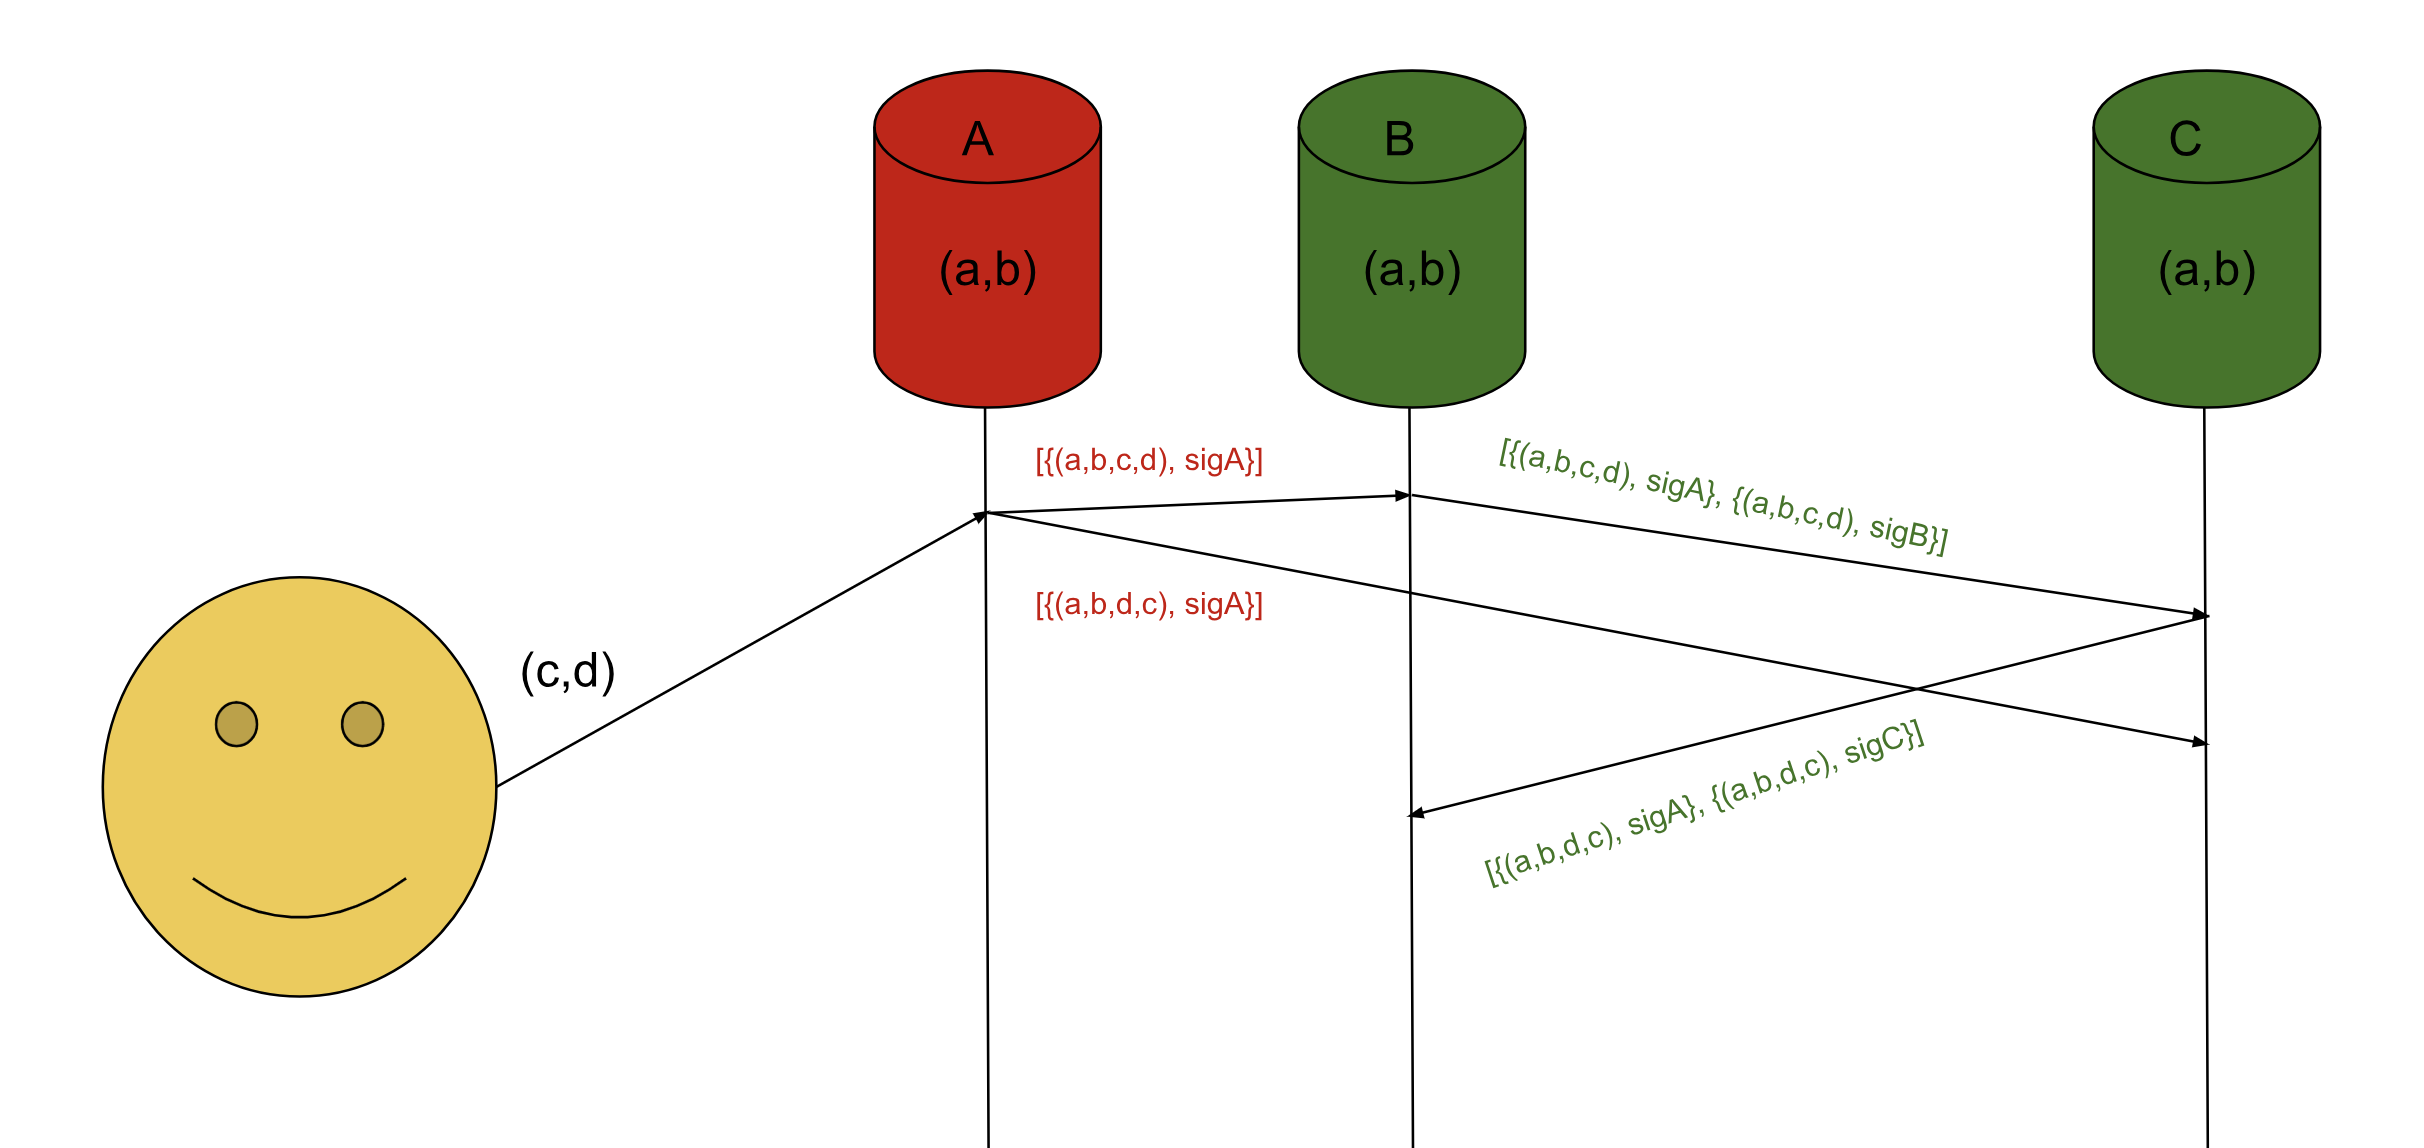
\includegraphics[width=\fscale{1}]{byz_faults.png}
	\caption{Byzantine fault detection during Paxos. Replica A sending conflicting messages is detected by B and C}
	\label{fig:byz_faults}
\end{figure}

\subsubsection{Sharding}
Picolo automatically partitions data into multiple shards when it grows too big for any one replica. Each shard consists of a set of key ranges (typically 64MB). A key range is the smallest atomic unit that is replicated aka governed by a paxos group. It is also the smallest unit of movement when data from one replica needs to be sharded into distinct replica sets. The process of sharding is a well studied problem in databases and implementations can be readily found, so we omit a detailed discussion here. 

\subsection{External consistency, distributed transactions \& hybrid time} \label{sec:hybrid_time}
Using atomic clocks, google external ntp service, stratum 1 ntp servers. Use logical time appended to physical time. Handle clock skew. Nodes that drift too apart should die. 
\newline\newline
\textbf{mvcc}: Keys have timestamps and queries can be made in the past or fetched from a snapshot in the past. Client configurable backup and restore mechanisms. How does this affect data sovereignty?

\subsection{Distributed query processing \& Dynamic clustering} \label{sec:dynamic_cluster}
High level architecture of a Picolo node looks like \figref{fig:node_arch}
\begin{figure}[h!] \centering
	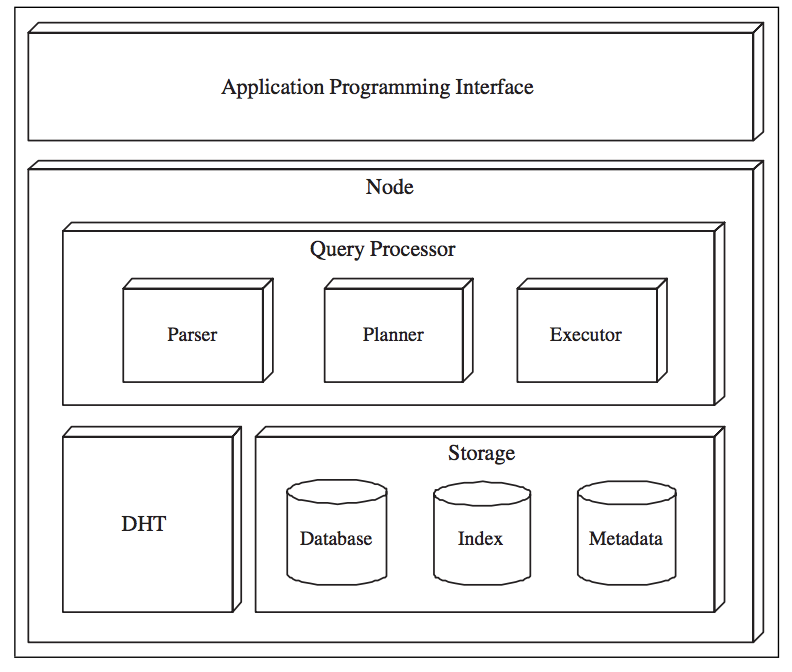
\includegraphics[width=\fscale{1}]{node_arch.png}
	\caption{A Picolo node}
	\label{fig:node_arch}
\end{figure}
The metadata depicted in the figure contains schema metadata to be exposed to the world. Nodes that wish to keep data private should not export the data's metadata to the metadata container. Suppose there is a table called \textit{users} with four columns: \textit{username}, \textit{firstname}, \textit{lastname} and \textit{email}. The exported metadata entry might look like:
\begin{center}
	\begin{tabular}{| c | c |} 
		\hline
		Entity & Keywords \\ [0.5ex] 
		\hline
		users & user, people, customer, profile\\ 
		\hline
		name & name \\
		\hline
		firstname & fn, {f\_name}, {first\_name} \\
		\hline
		lastname & ln, {l\_name}, {last\_name} \\
		\hline
		email & id, contact \\ [1ex] 
		\hline
	\end{tabular}
\end{center}
When a query is posed to any node in the system, the node first tries to fulfill it with a local query before passing it along to its neighbors. Remember, nodes in the system host data with heterogeneous schemas. Hence the keywords are used to find semantically similar data. Similarity metrics that determine whether a query matches a heterogeneous schema are not discussed here.
\newline\newline
\textbf{Dynamic clustering}
Semantic proximity metrics are used to find nodes that are hosting semantically similar schemas. Overtime, these nodes are discovered and are clustered together for better query performance by reducing the number of network hops required.

\subsection{Data sovereignty \& Access control} \label{sec:access_control}
Picolo supports two different schema types: \textit{application controlled} and \textit{user controlled}. Applications can use user controlled schemas to put users in absolute control of data and better comply with regulations like GDPR. For example, a decentralized twitter may  want users to have control over their tweets. Users can use any third party client or Picolo's official clients to interact with their tweets effectively rendering the decentralized twitter just another client to the data albeit with better features. \newline\newline
When semantics don't allow to put user in control of data, application controlled schemas can be used. An example here would be a decentralized ticketing application where users should not be given fine grained control to selectively delete data about which tickets they bought.
\newline\newline
\textbf{Access control} 
Applications and users may want to share data with other parties but may wish to impose access controls. There are a few ways of achieving this including building an API on top of the data or using proxy re-encryption techniques. We use a secret sharing scheme instead as it gels well with p2p nature of the system and does not introduce asymmetry like other solutions. Rules can be defined by a SQL like declarative language at any granularity desired like at the level of a single row or a cell. An example row level granularity rule looks like:\newline \newline
\texttt{SELECT  * \newline FROM users \newline WHERE email=foo@bar.com \newline NODE (SELECT nodeId FROM nodes WHERE domain=application)} \newline \newline
An example value level (only username is given access to) granularity rule looks like:\newline \newline
\texttt{ SELECT username \newline FROM users \newline WHERE email=foo@bar.com \newline NODE (SELECT nodeId FROM nodes)}\newline\newline
Here \texttt{NODE} is a new clause we introduce to SQL dialect.